\chapter{Necessary Mechanisms for Geo-Distributed Operation of Platform Services}
\begin{comment}
How to realize platform services at the edge?
    - describe core mechanisms needed
    - discuss how these mechanisms will enable efficient implementation of the aforementioned platform services in geo-distributed edge infrastructure
    - discuss the conceptual relationship of these mechanisms to the state-of-the-art in the cloud and other related research works
\end{comment}

\section{Introduction}
The challenges imposed by the peculiar characteristics of a geo-distributed Edge infrastructure on the design of  control-plane for platform services necessitate the introduction of novel mechanisms to address them. We propose three key mechanisms in this dissertation to address these challenges - Dynamic Spatial Context Management, Network Proximity Estimation and End-to-End Application Monitoring. The Dynamic Spatial Context Management mechanisms allows the control-plane of platform services to maintain a frequently updated view of the spatial context of system entities such as application instances, data-items and end-clients. This spatial context information is used to make control-plane decisions, such as mapping a client to an application instance, filtering the set of clients that need to share data for inter-client coordination, etc. While the Dynamic Spatial Context Management mechanism is used to establish logical connectivity between system entities based on spatial proximity, it is not responsible for mapping those system entities on to the physical infrastructure - a problem that requires infrastructure topology heterogeneity and timing considerations of applications to keep in mind. The Network Proximity Estimation mechanism allows control-plane policies to estimate the network latency between physical nodes in the infrastructure which can be used for the placement of system entities such that applications' requirements are satisfied. Finally, the continuous execution of applications requires that the control-plane monitor the end-to-end latency of each application instance, which includes several communication and computation components. The End-to-End Monitoring mechanisms allows the control-plane policies to obtain a time-aligned and aggregated view of the various component latencies making up the end-to-end observed latency so that the policies can detect a performance violation and perform a root-cause analysis to trigger the appropriate reconfiguration action to alleviate the violation. 
\par In this chapter, we will discuss the three mechanisms proposed in this dissertation in detail. For each mechanism, we will first describe the objective of the mechanism, enumerate examples of control-plane policies that will benefit from it, present the abstractions exposed to the control-plane policies, and why previous approaches at attaining this objective are not sufficient. Finally, we demonstrate the use of these abstractions for building useful control-plane policies that can support the efficient operation of platform services on a realistic Edge infrastructure against a workload of situation-awareness applications. Before we delve into the specifics of each mechanism, we present the scenario that has been considered to motivate the problems solved by these mechanisms and to design the experimental settings. 

\subsection{Infrastructure Topology considered}
\label{sec:nep_infra_topology}
\par To make the case for the mechanisms proposed in this dissertation, we utilize the dataset released by a previous work \cite{xu2021cloud}. The dataset characterizes the Edge cloud service of Alibaba Cloud, both at an infrastructure and a workload level. At the infrastructure level, it provides detailed information about the number of edge sites in each city and the network provider who owns them, the number and size of physical machines in each edge site and the network round-trip time between sites. At the workload level, the dataset contains information about the number and size of VMs hosted by each physical machine and the CPU utilization of each VM. For this evaluation, we focus on the city of Shanghai. We simulate client activity (including mobility) in the city of Shanghai, and thus to determine the network connectivity between a client and Edge site, the precise location of Edge Sites is needed. However, the dataset only provides a city-level granularity of Edge site locations. Hence, to approximate their precise geo-location, we gather the locations of cell towers owned by the different network providers from CellMapper \cite{cellmapper}, perform k-means clustering on them and obtain the likely location of the edge sites. The number of k-means clusters for each network provider's cell tower clustering is made equal to the number of Edge sites owned by that provider in Shanghai. After clustering is done, we order the Edge sites in the dataset by the number of physical resources they contain and the cluster centers by the number of celltowers in the cluster. We then map the Edge sites to the cluster centers in this order, to ensure that the sites with most physical resources serve the most number of cell towers, and so on. \cref{fig:shanghai_infra} illustrates the infrastructure topology, with the locations of cell towers and Edge sites marked. The physical infrastructure consists of Edge sites in Shanghai with fine-grained locations and sites in other cities in China, wherein their location is set to the center of that city. 

\begin{figure}
\centering
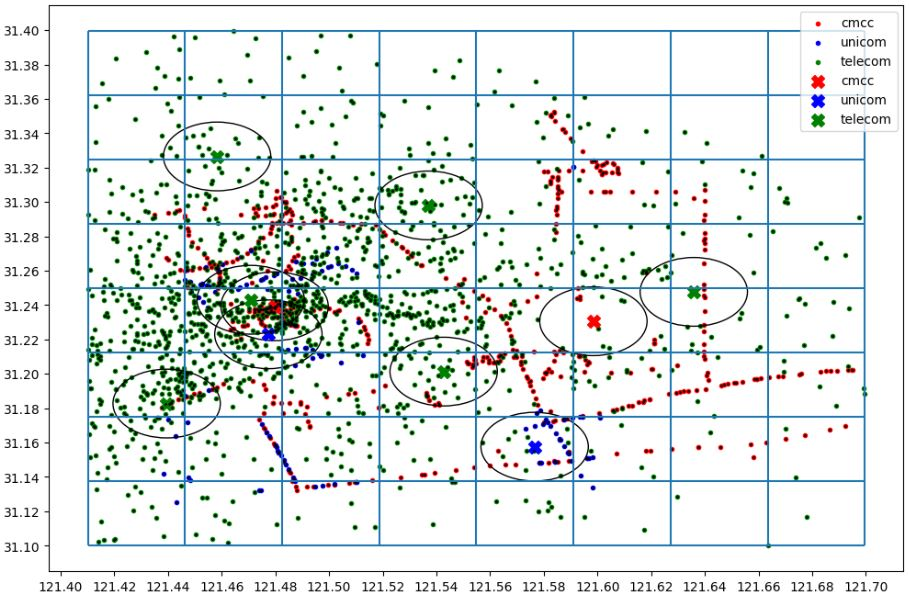
\includegraphics[width=0.5\textwidth]{figures/mechanisms/shanghai_infrastructure.JPG}
\caption{Edge infrastructure of the city of Shanghai which is under consideration in this chapter. The crosses denote Edge site locations, while the dots denote cell towers. \todo{Add lat-lng to the axes labels. Update the legend to be more meaningful.}}
\label{fig:shanghai_infra}
\end{figure}

\section{Dynamic Spatial Management}
\label{sec:spatial_ctx_mgmt}
\par Situation-awareness applications, e.g., collaborative autonomous driving and UAV swarm navigation, interact with the physical environment, by sensing and performing actions. Hence, the application instances that process sensor data and the data/state generated by them possess a spatial context, which ties them to the physical environment that they pertain to. The clients of such applications don't operate independently, but rather interact with each other. The information extracted from data sensed by one client is relevant for other clients because they could share the same spatial context. The set of other clients or data-items that a given client would be interested to coordinate with or access depends both on the spatial context of the given clients and that of the other clients and data-items. Such applications typically have an Area-of-Interest (AoI) that defines the spatial area within which a client would be interested in other clients or data-items. The AoI for an application is dependent on the nature of the application logic and clients. For instance, since vehicles in a city are not expected to move at speeds higher than a certain number, which limits how widespread relevant clients would be.
\par Such collaborative applications typically have an compute component that serves a number of clients that are meant to coordinate among each other. All clients connected to this component are able to share data among each other and coordinate. Similarly, collaborative applications also involve clients reading output data streams generated by other clients within their AoI. A large-scale deployment of such an application would necessarily have multiple instances of the compute component responsible for inter-client coordination running on multiple Edge sites, with each instance serving clients in a specific geographical region. Typically, the way to ensure that clients sharing a spatial context are processed by the same application instance (thus facilitating inter-client coordination) is to map clients in a specific geographical region to the same application instance. This property has been explained in a more general manner in \cref{sec:app_model_compute} and \cref{sec:app_model_comm}. Application instances and clients should also be able to query data items/streams and system entities with a spatial context that overlaps with their AoI. Doing so will enable inter-client coordination.
\begin{figure}
\centering
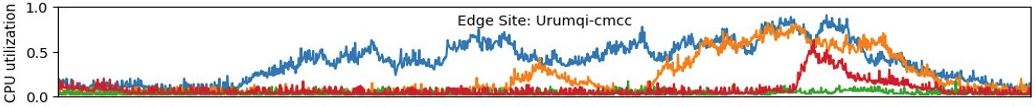
\includegraphics[width=\linewidth]{figures/mechanisms/spatial_ctx_mgmt/urumqi_cpu_util.JPG}
\caption{Variation of CPU utilization of multiple VMs running on the same Edge site owned by network provider CMCC in the city of Urumqi.}
\label{fig:vm_util}
\end{figure}
\par To ensure that each client is served by an application instance specific to its spatial context and that clients are able to query for data-items in their AoI, the spatial context of these entities needs to be maintained. The main challenge is to handle continuous client mobility, which results in the AoI and spatial context of each client to change continuously. Hence, a static mapping of clients to application instances does not work. Furthermore, clients need to continuously update the set of other clients and data-items in their AoI. Furthermore, given the continuous mobility of clients and the limited resource capacity of edge resources, workload skews are much more common. For instance, \cref{fig:vm_util} shows the variation of CPU utilization for VMs (each serving a specific geographical region) deployed on the same edge site. Such spatial workload skews would necessitate the monitoring and remapping of geographical regions to applications instances and data-items, so that the skews can be minimized and performance hotspots can be avoided.

\subsection{Control-plane policies that need this mechanism}
\par \textbf{Dynamic Client-Application Mapping. } Situation-awareness applications require that a client be connected to an application component that is assigned to the geographical area within which the client is currently located. A metric that quantifies the goodness of this mapping is Spatial Alignment, which measures how many of the expected clients that should have been mapped to an application component are actually mapped. The metric for spatial area $A$ is quantified in \cref{eq:spatial_alignment}.
\begin{equation}
SA \left( A \right) = \dfrac{\text{max. clients in }A\text{ served by same app instance}}{\text{number of clients in }A}
\label{eq:spatial_alignment}
\end{equation}
The control-plane policy for client-application mapping would ideally ensure the spatial alignment metric for all spatial areas is 1.0, meaning that all clients that are currently located in a given spatial area A are connected to the same application instance.

\par \textbf{Area-of-Interest Queries. } Clients and application components need to query system entities whose spatial context overlaps the querying entity's AoI. This query is served by the control-plane which evaluates the spatial context overlap with client's AoI and returns a list of satisfying system entities. We use a metric called AoI Satisfaction Rate to quantify the goodness of the query, as shown in \cref{eq:aoi_sat_rate}.
\begin{equation}
\text{AoI Satisfaction Rate} = \dfrac{|\{ e: e \text{ is returned by query  and } e \in AoI \}|}{|\{ e: e \in AoI \}|}
\label{eq:aoi_sat_rate}
\end{equation}
Ideally the control-plane policy for evaluating these queries should be able to achieve an AoI Satisfaction Rate of 1.0.
\subsection{Limitations of previous work in implementing policies}
Contemporary Edge computing solutions don't allow coordination among application components that are deployed across multiple Edge sites. Hence, a client $c$ that is mapped to an Edge site $E$ can only coordinate with other clients that are also mapped to the site $E$. Similarly, $c$ can only discover other system entities that are connected to the site $E$. We consider 2 broad ways in which clients have been mapped to Edge sites in previous work - mapping clients to the geographically closest site (GeoDist) and to the site with smallest RTT from the client (RTT). We show how both these approaches are deficient in satisfying the spatial alignment requirement of client-to-application mapping as well as serving Area-of-Interest based queries.

\begin{figure}
\centering
\begin{subfigure}{0.45\textwidth}
  \centering
  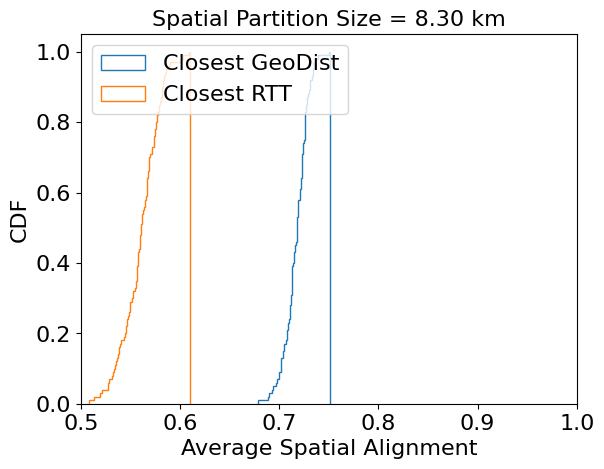
\includegraphics[width=\linewidth]{figures/mechanisms/spatial_ctx_mgmt/spatial_alignment_randomized_4_rows.png}
  \caption{}
\end{subfigure}%
\begin{subfigure}{0.45\textwidth}
  \centering
  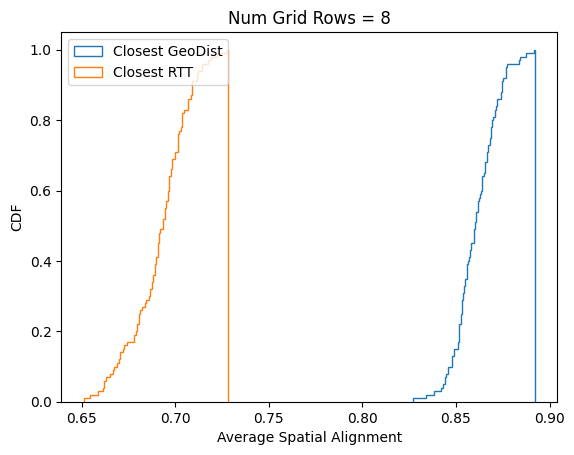
\includegraphics[width=\linewidth]{figures/mechanisms/spatial_ctx_mgmt/spatial_alignment_randomized_8_rows.png}
  \caption{}
\end{subfigure}\par\medskip
\begin{subfigure}{0.45\textwidth}
  \centering
  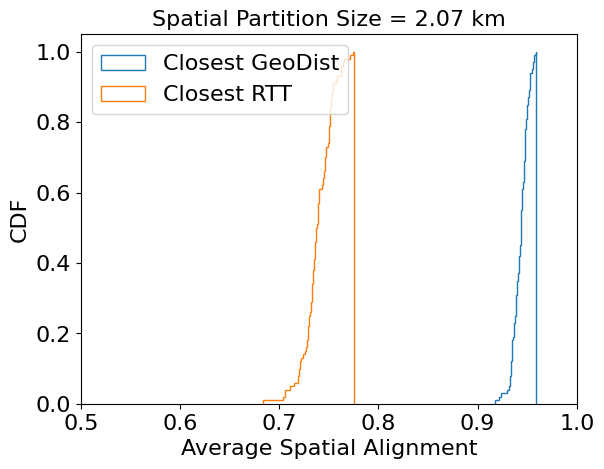
\includegraphics[width=\linewidth]{figures/mechanisms/spatial_ctx_mgmt/spatial_alignment_randomized_16_rows.png}
  \caption{}
\end{subfigure}%
\begin{subfigure}{0.45\textwidth}
  \centering
  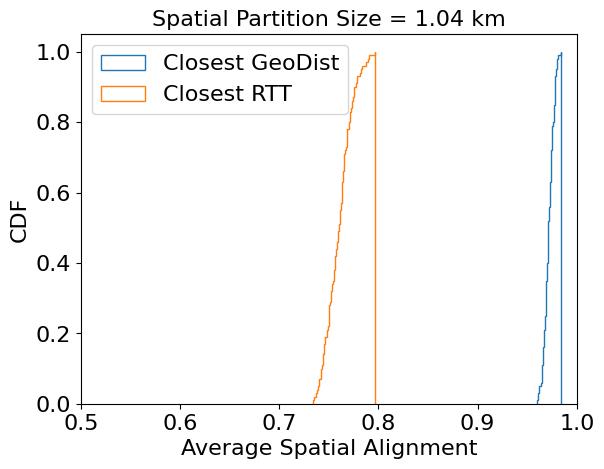
\includegraphics[width=\linewidth]{figures/mechanisms/spatial_ctx_mgmt/spatial_alignment_randomized_32_rows.png}
  \caption{}
\end{subfigure}
\caption{Spatial Alignment}
\label{fig:spatial_alignment_eval}
\end{figure}

To evaluate the above client-application mapping baseline heuristics in terms of spatial alignment, we first consider the area of the city under evaluation and divide it into a number of spatial areas, within which we ideally expect clients to be grouped and served by the same application instance (thereby creating a perfect spatial alignment). The number of spatial areas is varied in the experiment to represent a diverse set of applications. We create 1000 clients (with equal number of clients in each network provider) and place each one of them at a cell tower location. This client placement is randomized and the experiment is repeated 100 times. \cref{fig:spatial_alignment_eval} shows the distribution of the average spatial alignment that results from mapping clients to application instances using greedy heuristics that aim at minimizing geographical distance and network RTT between the client and Edge site. The metric shown is average spatial alignment, which is the average of the spatial alignment of all the spatial areas. Although the baseline policy GeoDist, which selects the geographically closest Edge site, is able to attain a high enough average spatial alignment, but doesn't attain the perfect 1.0 value because not all clients in a given geographical area always have the same Edge site to be the closest. Furthermore, the Closest RTT approach offers even worse spatial alignment because in a given spatial area, clients belonging to two different network providers are bound to be mapped to different sites. 

\begin{figure}
\centering
\begin{subfigure}{0.333\textwidth}
  \centering
  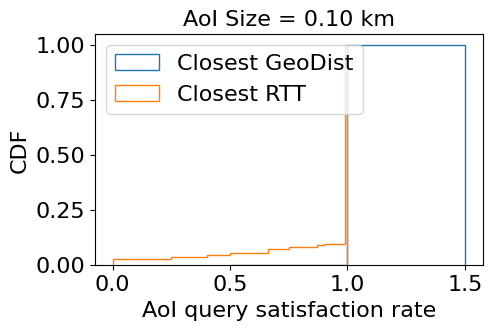
\includegraphics[width=\linewidth]{figures/mechanisms/spatial_ctx_mgmt/aoi_satisfaction_rate_cdf_AOI_0.100_km.png}
  \caption{}
\end{subfigure}%
\begin{subfigure}{0.333\textwidth}
  \centering
  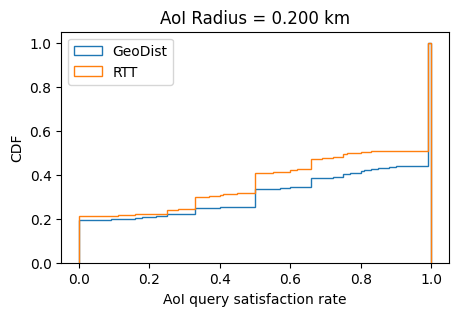
\includegraphics[width=\linewidth]{figures/mechanisms/spatial_ctx_mgmt/aoi_satisfaction_rate_cdf_AOI_0.200_km.png}
  \caption{}
\end{subfigure}
\begin{subfigure}{0.333\textwidth}
  \centering
  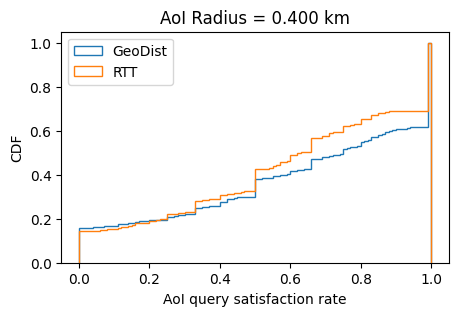
\includegraphics[width=\linewidth]{figures/mechanisms/spatial_ctx_mgmt/aoi_satisfaction_rate_cdf_AOI_0.400_km.png}
  \caption{}
\end{subfigure}
\par\medskip
\begin{subfigure}{0.333\textwidth}
  \centering
  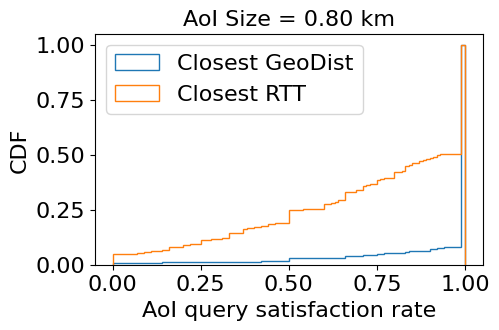
\includegraphics[width=\linewidth]{figures/mechanisms/spatial_ctx_mgmt/aoi_satisfaction_rate_cdf_AOI_0.800_km.png}
  \caption{}
\end{subfigure}%
\begin{subfigure}{0.333\textwidth}
  \centering
  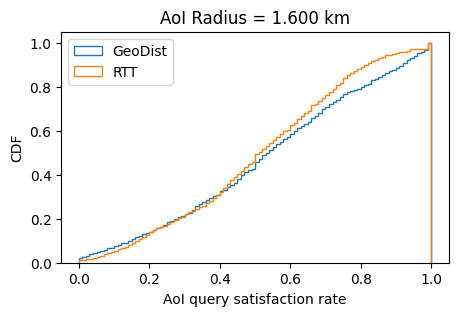
\includegraphics[width=\linewidth]{figures/mechanisms/spatial_ctx_mgmt/aoi_satisfaction_rate_cdf_AOI_1.600_km.png}
  \caption{}
\end{subfigure}%
\begin{subfigure}{0.333\textwidth}
  \centering
  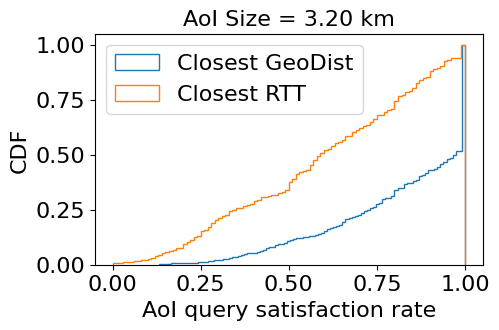
\includegraphics[width=\linewidth]{figures/mechanisms/spatial_ctx_mgmt/aoi_satisfaction_rate_cdf_AOI_3.200_km.png}
  \caption{}
\end{subfigure}
\caption{AoI Satisfaction Rate}
\label{fig:aoi_satisfaction_rate_eval}
\end{figure}

Next, \cref{fig:aoi_satisfaction_rate_eval} shows the distribution of AoI query satisfaction rate offered by the Closest GeoDist and Closest RTT baseline policies for retrieving the system entities with spatial context overlapping with the AoI of the querying client. For this evaluation, create 1 client at every cell tower location, and each client submits an AoI query to find which other clients are in its AoI. Depending on the client-Edge-site mapping, a variable number of AoI members are returned, which is compared with the actual set of clients within the AoI to compute the query satisfaction rate. The size of AoI query is varied to represent a diverse set of applications and their satisfaction rate distributions are shown.

\subsection{Interface exposed to the control-plane}
The Dynamic Spatial Context Management mechanism is utilized by both the centralized control-plane compute/data placement policy of platform services as well as the client library of the platform service running on the client application. The centralized control policy interacts with this mechanism to maintain the spatial context of the system entities (data and compute) while the client library uses this mechanism to keep track of the spatial context of clients. Both these types of spatial contexts are useful in determining which compute/data entities a given client would need to access. 
\par We divide the geographical space into rectangular regions called \textit{Tiles}, which are of arbitrary size. An example partitioning is shown in \cref{fig:example_partitioning}. Each Tile has a unique Tile ID, which can be used to directly reference the Tile. Each tile contains a number of entities, such as clients or data-items. In the following list, we enumerate the various functions that the mechanism exposes to the control-plane for accessing and updating this partitioning.
\begin{itemize}
\item \textbf{GetTileID}. This function takes a location as input and returns the ID of the Tile inside which that location falls.
\item \textbf{GetTileCoverage}. This function takes the ID of a tile as input and returns the bounding box which represents the spatial area covered by the tile.
\item \textbf{AddItemToTile}. This function assigns an item to a tile. If the item was previously assigned to a different tile, that association is deleted and association with the new tile (ID provided in input) is created.
\item \textbf{GetIntersectingTiles}. This function takes in a bounding box and returns the set of tiles that intersect with it. This function is useful for range queries.
\item \textbf{SplitTile}. This function call is used to split a tile into two. The split is carried out in a way to ensure that the number of entities in the two resultant tiles is (almost) equal. This function is used to handle load.
\item \textbf{HandleNewTile}. This is a callback function which needs to be handled by the control-plane when a new tile is created. 
\end{itemize}

\subsection{Demonstration of using the mechanism for implementing a control-plane policy}
We now demonstrate how the proposed mechanism is useful in implementing control-plane policies for platform services. For this mechanism, we use an application orchestrator as the driving example. \cref{algo:deploy_req} shows the pseudocode of the control-plane policy for finding a suitable application instance for mapping a client based on its geographical location and the spatial contexts of various application instances. The control-plane maintains a mapping between an application instance and the Tile which represents the geographical area served by the application instance. The policy first determines the Tile in which the client is currently located. If the client's tile already has an application instance associated with it, it returns connection information about that instance. Otherwise it deploys a new application instance for the client's tile, maps the application instance to the tile and returns its information to the client. The policy also adds the client to the tile to update the occupancy information, which can be used to detect overload and trigger re-partitioning.
\begin{algorithm}
\caption{Handling Deploy Request from Client}
\begin{algorithmic}
\Require client $c$
\Require client's location $loc$
\State $t \gets GetTileID \left( loc \right)$
\If{$APPS \left[ t \right] exists$}
    \State $A \gets APPS \left[ t \right]$
\Else
    \State Deploy app component $A$ for tile $t$
    \State $APPS  \left[ t \right] \gets A$
\EndIf
\State $AddToTile \left(t, c \right)$
\State $SendDeployReply \left(c, A \right)$
\end{algorithmic}
\label{algo:deploy_req}
\end{algorithm}

\cref{algo:handle_overloaded} describes the control-plane policy for handling an overloaded tile. This policy is triggered by the control-plane when it identifies that a given application instance is overloaded by the compute requirement of serving all the clients that are currently present in the tile its is serving. Hence, the tile needs to be split and workload divided among two application instances. The policy takes as input the tile associated with the overloaded application instance. The policy uses the \textit{SplitTile} function to create two new tiles. It reuses the application instance for the old tile for one of the new ones, and deploys another instance for the second new tile. Each client that belonged to the old tile is now a part of one of the two new tiles. The policy sends the connectivity information of the new application instances to the respective clients. 
\begin{algorithm}
\caption{Handling an Overloaded Tile}
\begin{algorithmic}
\Require overloaded tile $t$
\State $t1, t2 \gets SplitTile \left( t \right)$
\State $APPS \left[ t1 \right] \gets APPS \left[ t \right]$
\State Deploy app component $A$ for tile $t$
\State $APPS  \left[ t2 \right] \gets A$
\For{client $c \in GetEntities \left( t1 \right)$}
    \State $SendDeployReply \left(c, APPS \left[ t1 \right] \right)$
\EndFor
\For{client $c \in GetEntities \left( t2 \right)$}
    \State $SendDeployReply \left(c, APPS \left[ t2 \right] \right)$
\EndFor
\end{algorithmic}
\label{algo:handle_overloaded}
\end{algorithm}

\section{Network Proximity Estimation}
The performance perceived by applications when using platform services heavily depends on the mapping of compute and data components on the underlying physical infrastructure \cite{sarkar2016theoretical,amarasinghe2018data,naas2017ifogstor,liu2019mobility}. In a densely geo-distributed and heterogeneous infrastructure such as the Edge, the variation in communication latency caused by the choice of Edge Sites chosen to host compute or data components is significant. Therefore placement policies in the control-plane of platform services need to be aware of the topology of the underlying infrastructure to make their placement decisions. For instance, in the case of the collaborative perception application, the placement of application components should be such that the end-to-end processing latency is bounded under the specified threshold. Similarly, in the case of the drone swarm coordination application, the publish-subscribe topic should be placed on a suitable broker node to ensure that the end-to-end message delivery latency is bounded under the threshold.  
\par Therefore, the platform services require a mechanism that enables their control-plane to estimate the network latency between the end-clients and Edge Sites as well as across Edge Sites. Such a mechanism would be able to estimate the network latency between a pair of entities quickly and with low overhead, making it suitable to be used as a part of the placement policies of these platforms which evaluate a number of Edge Sites as candidates for compute or data placement. Given the dynamic nature of the Edge infrastructure and client mobility, the network proximity estimation should also be able to adapt to dynamic changes in network latency between system entities.

\subsection{Control-plane policies that need this mechanism}
Network proximity estimation is useful by control-plane policies that map logical system entities, such as application instances or publish-subscribe topics, to physical nodes in a way that the end-to-end latency requirements of applications are met. Previous work in this space \cite{amarasinghe2018data,naas2017ifogstor,liu2019mobility} relies on inter-node communication latency estimates for making these decisions, however does not go into detail about how these estimates are obtained. For the application orchestrator platform service, where an application instance consists of a pipeline of multiple components, the end-to-end latency is the sum of the processing latency at each application component and the communication latency between each upstream-downstream pair of components. Similarly, in the case of a publish-subscribe system, the end-to-end messaging latency for a given topic is the sum of the communication latency from the publisher clients to the broker, the processing latency on the broker and the communication latency from the broker to the subscriber clients. In the above two systems, estimating the processing latency of application components and publish-subscribe broker can be done using previous works in the cloud computing realm as well \cite{khare2018scalable}. However, for estimating the communication latency between a pair of nodes requires the proposed mechanism. Hence, the application placement policy for the orchestrator and topic placement policy for publish-subscribe system can benefit from the proposed mechanism. 

\subsection{Limitations of previous work in proximity-aware compute/data placement}
Control-plane policies for ensuring that compute and data entities accessed by a given set of clients is placed in their proximity have been one of the main directions of previous research in edge computing. The use of geographical distance as a proxy for network latency has been commonly used, given the simplicity of the scheduling logic once the geolocations of system entities (e.g., clients and edge sites) is known. Sarkar and Misra \cite{sarkar2016theoretical} propose the transformation of geographical distance between client and candidate edge site into the network latency between them using a linear transformation $rtt\left(ms\right) = dist \left(km\right) * 0.02 + 5$ \cite{qureshi2010power}. Other works don't rely on the use of such a transformation, but rather perform greedy placement on the geographically closest site to ensure efficient access. Geographical location has also been used in a much more coarse-grained manner, in which the placement of compute/data entities is specified to be a large location, e.g., within a city \cite{vilaccageolocate}. The selection of the specific edge site is done on the basis of another policy logic that aims to ensure even load distribution among the various edge sites in a given geographical area.
\par The above approaches fail to work in realistic edge settings because they assume that geographical proximity is correlated with network proximity, which is not true because of lack of uniformity in the way in which different network providers are peered with each other. Two systems entities in close physical proximity might have to communicate through extended routing paths because of the peering between the network providers serving the two entities. In \cref{fig:geodist_vs_rtt}, we present the variation of network round-trip time between an edge site located in Shanghai to other edge sites throughout China. It shows that although network latencies are loosely correlated with geographical distance, there is a significant amount of variance, which will result in control-policies choosing an incorrect edge site for compute/data placement. In \cref{fig:same_city_diff_prov}, we specifically measure the network round-trip times between sites that are located in the same city, but are part of different network providers. The high round-trip times are reason to assume that the high variation in \cref{fig:geodist_vs_rtt} is due to the expensive peering between different network providers hosting edge sites. 
\begin{figure*}[t!]
    \centering
    \begin{subfigure}[t]{0.45\textwidth}
        \centering
        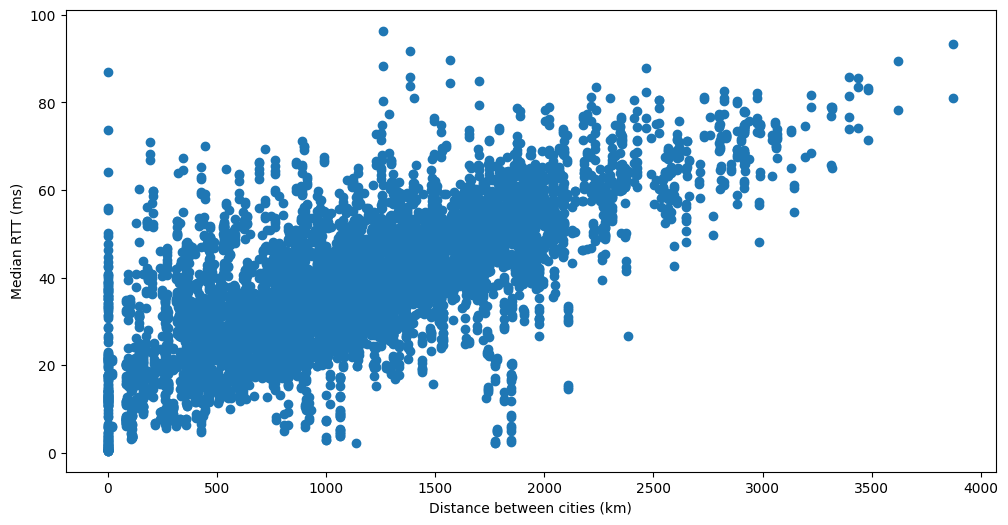
\includegraphics[width=\textwidth]{figures/mechanisms/nw_proximity/shortest-rtt-vs-dist.png}
        \caption{Variation of network RTT with geographical distance between Edge Sites.}
        \label{fig:geodist_vs_rtt}
    \end{subfigure}%
    ~ 
    \begin{subfigure}[t]{0.45\textwidth}
        \centering
        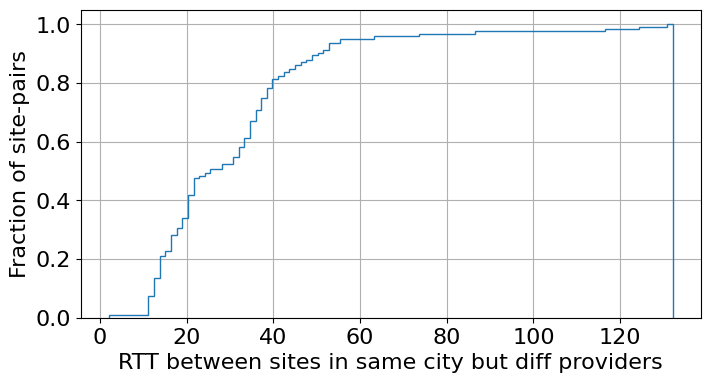
\includegraphics[width=\textwidth]{figures/mechanisms/nw_proximity/same_city_diff_provider_rtts.png}
        \caption{Client-Site RTT for sites selected by transforming the geographical distance into network RTT and uniformly choosing one among the set of sites satisfying the latency constraint.}
        \label{fig:same_city_diff_prov}
    \end{subfigure}
    \caption{Variation of network RTT between edge sites with respect to geographical distance.}
\end{figure*}

\begin{figure*}[t!]
    \centering
    \begin{subfigure}[t]{0.45\textwidth}
        \centering
        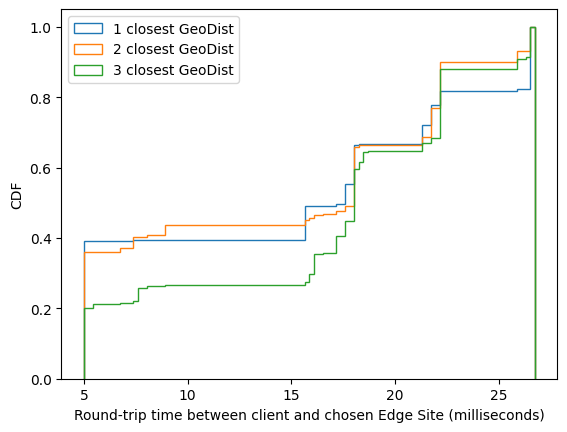
\includegraphics[width=\textwidth]{figures/mechanisms/nw_proximity/geodist_greedy.png}
        \caption{Client-Site RTT for sites selected by Greedy approaches. In the case that the closest site is overloaded, the next closest site is considered and so on.}
        \label{fig:geodist_greedy}
    \end{subfigure}%
    ~ 
    \begin{subfigure}[t]{0.45\textwidth}
        \centering
        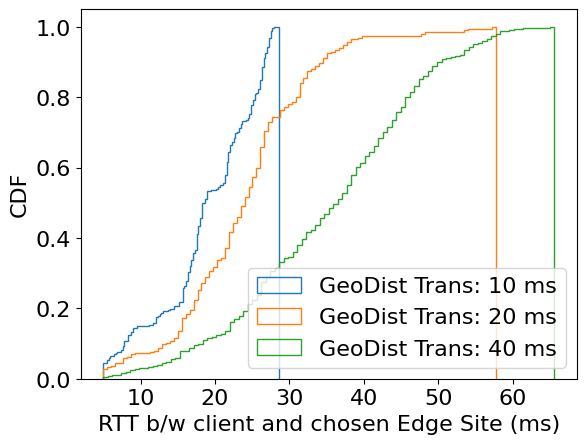
\includegraphics[width=\textwidth]{figures/mechanisms/nw_proximity/geodist_trans_rtt.png}
        \caption{Client-Site RTT for sites selected by transforming the geographical distance into network RTT and uniformly choosing one among the set of sites satisfying the latency constraint.}
        \label{fig:geodist_trans}
    \end{subfigure}
    \label{fig:baseline_proximity_policies}
    \caption{Performance of Edge Site selection approaches that rely on geographical distance as a proxy for network proximity.}
\end{figure*}

\par We evaluate the efficacy of the aforementioned baseline proximity estimation techniques - the greedy distance-minimization approach and the one that transforms geographical distance to network RTT. For this experiment, we consider the infrastructure topology of the city of Shanghai as described in \cref{sec:nep_infra_topology}. We simulate clients at randomly (uniformly) chosen cell tower locations and aim to find an Edge site to host its application instance using one of the above two policies. The goodness of an edge site selection is quantified by the observed RTT between the client and chosen edge site. 
\par The Greedy policy always selects the closest Edge site in terms of geographical distance between the client and the site. In case the chosen Edge site is undergoing compute overload, the policy selects the next closest site, and so on. The other site selection policy that we evaluate is one that transforms the geographical distance between client and edge site to network round-trip time and uses this estimate to filter out those sites that can meet the latency bound imposed by the application. Among the filtered sites, the policy uniformly selects one so as to minimize workload skews.
\par \cref{fig:geodist_greedy} shows the observed RTT when selecting site using the greedy approach. For more than 50 percent of the clients, the geographically closest site is not the one that it is directly connected to over the network, and hence, traffic needs to go through the network provider's core, or through the Internet to get to the selected site. Since there is no correlation between geographical distance and network RTT, this behavior is similar for 2nd and 3rd closest sites as well. For the distance-RTT transformation based approach, we compare the site selection with an application-imposed RTT bound of 10, 20 and 40 milliseconds. We see however, that the transformation does not sufficiently filter out infeasible sites and a large majority of clients have the bound violated.

\subsection{Interface provided to control-plane}
All system components of the platform service (clients, worker nodes, data nodes, etc.) are assigned a unique network proximity identifier. The network proximity mechanism then provides the platform service a function \textbf{NetworkRTT} which takes as input the IDs of two system components and returns the estimated network round-trip time between the two components. 

\subsection{Using network proximity mechanism for compute/data placement}
We now demonstrate the use of the proposed Network Proximity Estimation mechanism for implementing a control-plane policy, specifically the broker selection policy for a publish-subscribe system. This control-plane policy selects the broker to host a given topic such that the end-to-end message delivery latency for all publisher-subscriber pairs is under the latency threshold for the topic. It iterates over all the potential brokers and computes the worst-case communication latency if the topic is hosted on each of those brokers. The worst-case communication latency is the sum of the maximum publisher-broker network latency and the maximum broker-subscriber network latency. The sum of worst-case communication latency and processing latency on the broker gives the worst-case end-to-end latency for that topic. All the brokers that have the worst-case end-to-end latency under the topic-specific threshold are selected as candidates. The policy finally selects the candidate currently serving the lowest message rate among all candidates to ensure load balancing among brokers.

\begin{algorithm}
\caption{Broker selection policy for topic $T$ with end-to-end latency threshold $L_{th}$}
\begin{algorithmic}
\Require topic $T$
\Require latency threshold $L_{th}$
\State $prod \gets \text{ set of producers for }T$
\State $cons \gets \text{ set of consumers for }T$
\State $candidates \gets \{\}$
\For{$\text{each broker } b$} 
    \State $nw\_lat \gets max_{p \in prod} \dfrac{1}{2} \cdot NetworkRTT \left( p, b \right) + max_{c \in cons} \dfrac{1}{2} \cdot NetworkRTT \left( c, b \right)$
    \State $e2e \gets nw\_lat + proc\_latency \left( b \right)$
    \If{$e2e \leq L_{th}$}
        \State $candidates \gets candidates \cup \{b\}$
    \EndIf
\EndFor
\Return broker in $candidates$ with lowest $msg\_rate$
\end{algorithmic}
\end{algorithm}

\section{Distributed End-to-End Monitoring}
Situation-awareness applications require that the end-to-end latency and spatial affinity requirements are satisfied for the entire lifetime of the application, so that correct functionality can be guaranteed. However, given the constant mobility of end-clients, these requirements are likely to be violated repeatedly and frequently. For instance, a car moving away for the Edge Site currently serving the vehicle-local processing component would incur higher end-to-end processing latency. Similarly, a vehicle that moves out of the geographical area being served by the current region-level application component would receive fused sensor data updates that no longer pertain to its spatial context. Hence, the control-plane of the platform services are required to constantly monitor the running applications for such violations, perform root-cause analysis for determining the cause of the violation, and take appropriate reconfiguration action(s) to resolve the violation. Examples of such a reconfiguration would be the migration of the application component to an Edge Site that is closer (in terms of network proximity) to the end-client to ensure end-to-end latency satisfaction, or the re-mapping of the end-client to an application component that has the same spatial context as the end-client to satisfy the spatial affinity requirement.
\begin{figure}
\centering
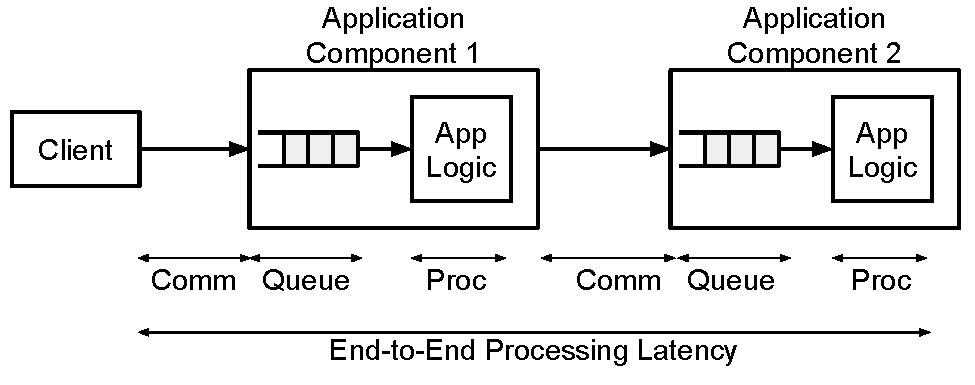
\includegraphics[width=0.75\linewidth]{figures/mechanisms/monitoring/pipeline_latencies}
\caption{A breakdown of the end-to-end processing latency of an application pipeline into its constituent latencies.}
\label{fig:pipeline_latencies}
\end{figure}
\par Thorough monitoring of applications running atop platform services is a non-trivial task because there can be multiple sources of performance violation. For instance, as shown in \cref{fig:pipeline_latencies}, the observed end-to-end latency of the application instance is a sum of the queuing, execution and downstream communication latencies of each operator in the pipeline.  Thus, in order to detect a violation of the end-to-end latency requirement and identify the root-cause requires the monitoring of all the component latency metrics as independent timeseries and their aggregation and analysis. Furthermore, each platform service has its own set of metrics that need to be monitored for each application instance. These metrics than need to be aggregated and analyzed in a platform service-specific way as well to detect violations. The monitoring mechanism needs to scale with an increasing number of application instances being monitored and impose low overhead on the applications and infrastructure.

\subsubsection{Shortcomings of previous work}
\par Application monitoring has been an active area of work in the cloud computing space with a number of research projects and commercial offerings available. In the context of cloud computing, applications typically don't possess end-to-end latency requirements and the goal of monitoring is to ensure that the tail latency of a given service (that could consist of multiple instances) doesn't increase significantly. Platforms such as Prometheus \cite{prometheus} and Monasca \cite{monasca} don't support the aggregation of multiple metrics to study the behavior of end-to-end latency. Furthermore, their architecture is a fully centralized one, resulting in the use of network bandwidth to send the monitoring data to the cloud.
\par Monitoring systems designed for edge computing environments also suffer from limitations, wherein they aggregate measured metrics over geographical regions instead of aggregating multiple metrics pertaining to the same application instance \cite{fmone, gonccalves2021dynamic}. Such systems are not likely to detect violations of end-to-end performance constraints. Previous contributions to building systems services such as publish-subscribe systems \cite{emma} and distributed application runtimes \cite{foglets} consist of monitoring subsystems that only monitor the the network connectivity between a client and the edge site that it is connected directly to. Since these solutions don't consider end-to-end latency as the primary metric, they would result in triggering more reconfigurations to keep clients connected to the closest edge site than needed.
\begin{figure}
\centering
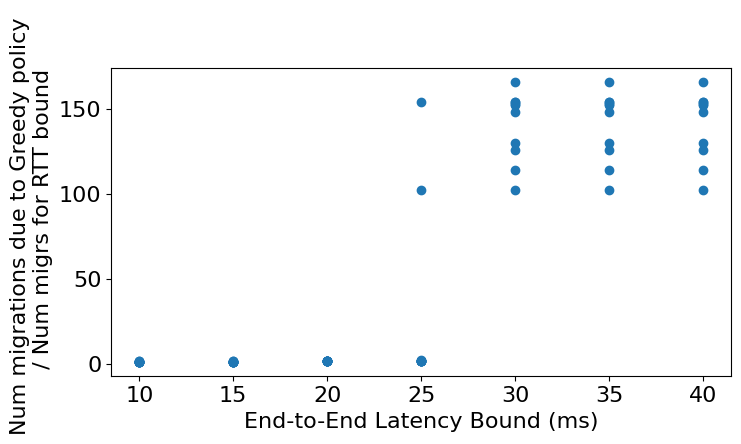
\includegraphics[width=0.75\linewidth]{figures/mechanisms/monitoring/migrations_count.png}
\caption{Ratio of the number of migrations triggered by Greedy monitoring scheme versus those triggered by an optimal policy. The end-to-end latency threshold is varied along the x-axis.}
\label{fig:migration_count}
\end{figure}
\par In the following we show an evaluation of a greedy monitoring approach that aims to minimize the last-mile network latency between the client and the edge-site it directly connects to. The metric of interest is the number of migrations triggered by such a policy compared to an optimal policy that monitors the end-to-end latency and only triggers a migration when it is violated. We simulate the mobility of 200 independent clients in the city of Shanghai using the Random Waypoint mobility model and track the number of migrations triggered by both the greedy and optimal policies. In \cref{fig:migration_count}, we present the ratio of the migrations triggered by the greedy policy and that by the optimal policy with increasing end-to-end latency bound. We see that as the end-to-end latency bound increases, the relative number of migrations triggered by greedy policy becomes much higher. This is because, although the greedy policy triggers the same number of migrations as it is independent of the end-to-end latency constraint, the number of migrations triggered by the optimal policy decreases with an increase in the threshold. This necessitates that any useful and efficient monitoring system should look at end-to-end latency observed by applications and not individual component latencies.

\subsection{Interface provided to control-plane}
The following abstractions are provided to the control-plane of a platform service when using the distributed end-to-end monitoring mechanism.
\begin{itemize}
\item \textbf{RegisterAppUnit.} Registration of an Application Unit when it is created. For instance, when a new topic is created in a publish-subscribe system, the topic should be registered as a new Application Unit.
\item \textbf{RegisterMetric.} System components can register custom metrics and publish measurements to them. The metrics are annotated with the application unit that they correspond do, as well as custom platform-specific tags. The following snippet shows an example, which measures the network coordinate of a consumer client $C1$ for topic T.
\begin{minted}{yaml}
-   entity_id : "L10"
    entity_type: "APP"
    root_component: "L0"
    metric: "net_latency"
\end{minted}
Each metric stream is represented an ordered sequence of measurements along with their timestamps as shown in \cref{eq:metric_stream}.
\begin{equation}
M = \left[ \cdots , \left( t, v \right) , \cdots \right] \text{ where } 0 < t < \infty
\label{eq:metric_stream}
\end{equation}

\item \textbf{AlignMetrics.} The control-plane policy can time-align the measurements for a specific metric into well-defined buckets. This interface is necessary as a preprocessing step before multiple metrics can be aggregated together. Since different metrics are likely to be recorded at different instants in time, aligning them in time allows the values from different metrics to be processed together, such that two values from different metrics that were collected at roughly the same time can be processed together. \cref{fig:time_alignment} illustrates the time alignment of a metric for a fixed size time bucket, and all measurements within a given bucket are aggregated by taking an average over them. The platform service is supposed to provide the bucket size $B$ and the aggregation function $func$ for aggregating a metric $M$.
\begin{figure}
\centering
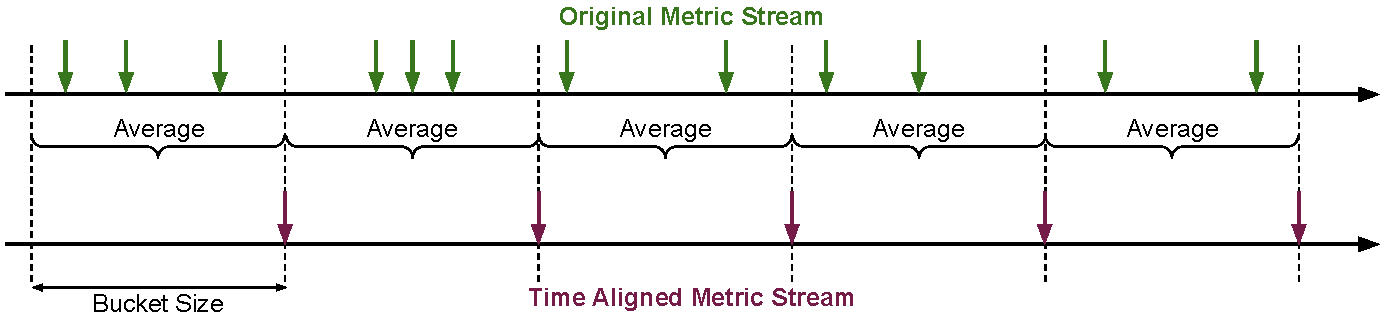
\includegraphics[width=\linewidth]{figures/mechanisms/monitoring/time_alignment}
\caption{Illustration of time alignment of metrics. The individual measurements within each time bucket are aggregated using average function to generate the measurement for that bucket. The time alignment function takes as input a metric stream and time bucket size and returns another stream.}
\label{fig:time_alignment}
\end{figure}
\begin{multline}
ALIGN^{func}_{B} \left( M \right) = \left[ \cdots , \left( t, v \right) , \cdots \right] \text{ where } t = n\cdot B \text{ and } 0 < n < \infty \\ \text{ and } v = func \left( \{ v' : \left( t', v'\right) \in M \text{ and } B\cdot \left( n-1\right) < t' \leq n \cdot B \} \right)
\label{eq:metric_stream}
\end{multline}

%\item Platform-specific definition of the system entity processing all the metrics of a given application unit for performing aggregation and violation detection. For instance, in the case of a publish-subscribe system, all the metrics pertaining to a specific topic can be processed at the broker serving that topic.
\item \textbf{ProcessMetrics. }Support platform-specific logic for metrics aggregation and violation detection policies. The logic should be able to query metrics using the aforementioned tags, generate new aggregated metrics, and call an endpoint in the platform service's control-plane to trigger a reconfiguration upon detecting performance violation. The policy should also be able to access certain configurations of the platform service, such as the mapping of child application components to parent application component for the application orchestrator, or the mapping of topics to brokers in the case of publish-subscribe system. Information about such configurations is useful for knowing which metrics need to be aggregated together.
\end{itemize}

\subsection{Demonstration of using end-to-end monitoring for control-plane policy of a platform service}
In this section, we show how the end-to-end monitoring mechanism will be used for implementing the control-plane policy for detecting violation of end-to-end processing latency for a geo-distributed application orchestrator system. For this example, we would restrict the discussion to clients and broker for a single application instance, but the approach generalizes to multiple instances.
\begin{enumerate}
\item The library of the platform service running alongside each client and backend application instance generates two metrics - namely the processing latency and network latency to the parent application instance. For application component $e$ denote them as $proc_e$ and $net_e$.\\
\begin{minipage}{0.45\textwidth}
\begin{minted}{yaml}
-   entity_id : "L20"
    entity_type: "CLIENT"
    root_component: "L0"
    metric: "proc_latency"
\end{minted}
\end{minipage}%
\hfill
\begin{minipage}{0.45\textwidth}
\begin{tabular}{p{\textwidth}}
\begin{minted}{yaml}
-   entity_id : "L10"
    entity_type: "APP"
    root_component: "L0"
    metric: "net_latency"
\end{minted}
\end{tabular}
\end{minipage}%

\item The control-plane policy for detecting violations of end-to-end processing latency performs calculations for each of the root application instances, which we denote as $L_0$. It selects the latency metrics corresponding to the clients that are connected to $L_0$ as shown in \cref{fig:app_pipeline}. It uses a query like the following to select the latency metrics for all the clients that are connected to the root application component $L_0$.
\begin{minted}{sql}
SELECT METRICS WITH entity_type="CLIENT" AND app_unit="L0"
\end{minted}
\begin{figure}
\centering
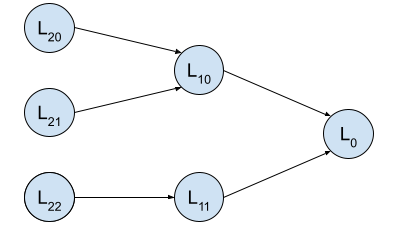
\includegraphics[width=0.5\textwidth]{figures/mechanisms/monitoring/app_pipeline.png}
\caption{Schematic of a typical situation-awareness application. The application model resembles a tree, with the leaf vertices corresponding to clients. Each vertex has a parent vertex except the root vertex.}
\label{fig:app_pipeline}
\end{figure}
\item The above set of metrics are then grouped by the field $entity\_ID$ because they contain both processing latency and network latency metrics for each client. Grouping them by $entity\_ID$ allows the policy to separate the metrics of a specific client from other clients.
\item For each client component $c$, the policy computes the set of application components $S_c$ that process data generated by $c$. The following pseudocode illustrates this computation.
\begin{algorithmic}
\State $n \gets c$
\State $S_c \gets \{\}$
\While{$n \neq \phi$} 
    \State $S_c \gets S_c \cup \{ n \}$
    \State $n \gets M \left[ n \right]$
\EndWhile
\end{algorithmic}
We use the notation $M \left[ n \right]$ to denote the parent application component serving $n$. The parent of the root application component is designated to be null ($\phi$).

\item The policy time-aligns all the metric streams using the function $ALIGN^{AVG}_{5secs}$ We denote the aligned version of metric stream $M$ as $M*$.

\item For each client $c$, now it is possible to compute a time-aligned metric stream which records the end-to-end processing latency for $c$.
\begin{equation}
E2E_c^* = \sum_{e \in S_c} proc_e^* + net_e^*
\end{equation}

\end{enumerate}

